
%%%%%%%%%%%%%%%%%
%%%%%%%%%%%%%%%%%
\begin{frame}
	\shiftedframetitle{4. Implementation}
\begin{minipage}{0.35\textwidth}
\begin{tcolorbox}[title= \textbf{Mapping setups}, colframe=TUMOrange,
colback=TUMOrange!30] 
\begin{table}[]
\begin{tabular}{ll}
Supercritical & $2D$ SWE  $\rightarrow$  $2D$ SWE     \\ 
Subcritical   & $2D$ SWE  $\rightarrow$  $2D$ SWE     \\[0.3cm]
Supercritical & $2D$ SWE  $\rightarrow$  $3D$ OF      \\ 
Subcritical   & $2D$ SWE  $\rightarrow$  $3D$ OF      \\[0.3cm]
Supercritical & $3D$ OF   $\rightarrow$  $2D$ SWE     \\ 
Subcritical   & $3D$ OF   $\rightarrow$  $2D$ SWE     \\[0.3cm]
Supercritical & $3D$ OF   $\rightarrow$  $3D$ OF      \\ 
Subcritical   & $3D$ OF   $\rightarrow$  $3D$ OF      \\ 
\end{tabular}
%\caption{Mapping setups}
%\label{table:1}
\end{table}
\end{tcolorbox}
\end{minipage}
\hspace{1cm}
\begin{minipage}{.55\textwidth}
\addtolength{\leftmargini}{-0.8cm}
\begin{itemize}
\item<2->[]
\begin{tcolorbox}[title= \textbf{Supercritical Cases}, colframe=TUMGreen,
colback=TUMGreen!30] 
\begin{table}[!h]
\centering
\begin{tabular}{lll}
\textbf{Case / Domain} & \textbf{Left domain} & \textbf{Right domain} \\[0.3cm]
\textbf{SWE $\rightarrow$ SWE} & Radial breaking dam      & Surface at rest      \\[0.1cm]
\textbf{SWE $\rightarrow$ OF}  & Radial breaking dam x2   & Surface at rest      \\[0.1cm]
\textbf{OF $\rightarrow$ SWE}  & Radial breaking dam   & Surface at rest   \\[0.1cm]
\textbf{OF $\rightarrow$ OF}   & Breaking dam      & Empty domain
\end{tabular}
%\caption{Scenarios for each setup on supercritical flow.}
%\label{t:condsSup}
\end{table}
\end{tcolorbox}
\item<3->[]
\begin{tcolorbox}[title= \textbf{Subcritical Cases}, colframe=TUMDarkBlue,
colback=TUMDarkBlue!30]
\begin{table}[!h]
\centering
\begin{tabular}{lll}
\textbf{Case / Domain} & \textbf{Left domain} & \textbf{Right domain} \\[0.3cm]
\textbf{SWE $\rightarrow$ SWE} & Radial breaking dam      & Radial breaking dam      \\[0.1cm]
\textbf{SWE $\rightarrow$ OF}  & Flow to the right & Surface at rest with wall        \\ [0.1cm]
\textbf{OF $\rightarrow$ SWE}  & Flow to the right & Surface at rest with wall      \\[0.1cm]
\textbf{OF $\rightarrow$ OF}   & Breaking dam      & Empty domain with wall
\end{tabular}
%\caption{Scenarios for each setup on subcritical flow.}
%\label{t:condsSub}
\end{table}
\end{tcolorbox}

\end{itemize}
\end{minipage}
\end{frame}


\begin{frame}
%TODO improve this slide
\shiftedframetitle{\large Boundary Conditions}
\begin{figure}
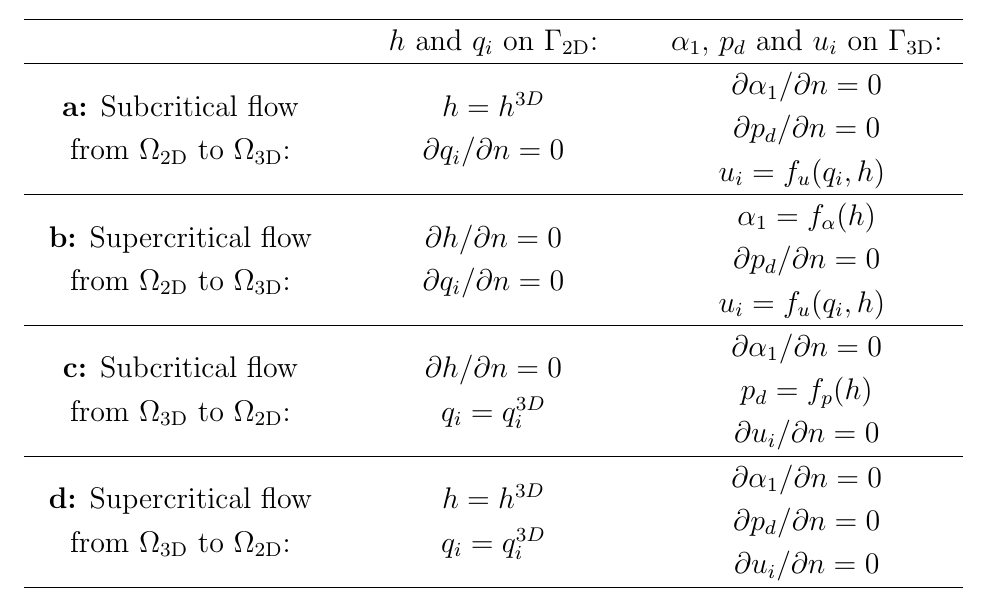
\includegraphics[scale=0.44]{Resources/Images/bcs_mintgen.png}
\caption{Boundary conditions \cite{mintgen}}
\end{figure}
\end{frame}

